\documentclass[12pt]{article}
\usepackage[brazilian]{babel}
\usepackage[utf8]{inputenc}
\usepackage{setspace}
\usepackage{boxedminipage}
\usepackage{amsmath}
\usepackage{latexsym}
\usepackage{multirow}
\usepackage[pdftex]{graphicx}
\usepackage{float}
\usepackage{url}
\usepackage{tikz}
\usetikzlibrary{bayesnet}
\usepackage{blkarray}

\renewcommand{\familydefault}{\sfdefault}
\newcommand{\question}[2] {\vspace{0.3in}\noindent{\subsection*{Exercício #1. #2} \vspace{0.15in}}}
\renewcommand{\part}[1] {{\vspace{0.15in}\noindent\textbf (#1)} \vspace{0.10in}}
\newcommand{\answer}[1]{{\fontfamily{\rmdefault}\selectfont \textbf{R:} #1}}
\newcommand{\overbar}[1]{\mkern 2mu\overline{\mkern-2mu#1\mkern-2mu}\mkern 2mu}

%\setlength{\parskip}{0.1cm}
\setlength{\paperheight}{29.7cm}
\setlength{\textheight}{23.0cm}
\setlength{\textwidth}{16.5cm}
\setlength{\oddsidemargin}{0.0cm}
\setlength{\topmargin}{-1.0cm}
\pagestyle{empty}


\begin{document}
\title{Lista de exercícios de Introdução à Redes Booleanas Probabilisticas}
\author{\large Gustavo Estrela de Matos}
\date{\today}
\maketitle

\question{1}{Dada a rede booleana abaixo:}
\begin{center}
\begin{tikzpicture}
  \tikzstyle{gene} = [circle, minimum width=8pt, draw, inner sep=0pt]
  % Define nodes
  \node[gene, label={[yshift=0.1cm] $x_1$}] (x1) {};
  \node[gene, right=2cm of x1, label={[yshift=.1cm] $x_2$}] (x2) {};
  \node[gene, below=2cm of x2, label={[yshift=-1cm] $x_4$}] (x4) {};
  \node[gene, below=2cm of x1, label={[yshift=-1cm] $x_3$}] (x3) {};

  \edge [->, shorten >=.1cm] {x1}{x2};
  \edge [-Bar, shorten >=.1cm] {x4}{x2};
  \edge [->, shorten >=.1cm] {x3}{x4};
  \edge [-Bar, shorten >=.1cm] {x3}{x1};
  \edge [->, shorten >= .1cm] {x2}{x3}
 \end{tikzpicture}
\end{center}

\part{1} Monte a matriz de interação.

\answer{
\[
\begin{blockarray}{ccccc}
x_1 & x_2 & x_3 & x_4 \\
\begin{block}{[cccc]c}
  0 & 0 & -1 & 0  & x_1 \\
  1 & 0 & 0 & -1  & x_2 \\
  0 & 1 & 0 & 0  & x_3 \\
  0 & 0 & 1 & 0  & x_4 \\
\end{block}
\end{blockarray}
\]
}

\part{2} Para cada gene, encontre sua expressão booleana

\answer {

Para $x_1$:

\begin{tabular}{c l}
$\begin{array}{cc | c}
  x_1 (t) &  x_3 (t) & x_1 (t + 1) \\
  \hline
    0     &     0    &     0       \\
    0     &     1    &     0       \\
    1     &     0    &     1       \\
    1     &     1    &     0       
\end{array}$

&

Portanto, $x_1 (t + 1) = x_1 (t) \bar x_3 (t)$ 
\end{tabular}


\vspace{.2cm}
Para $x_2$:

\begin{tabular}{c l}
$\begin{array}{ccc | c}
  x_2 (t) &  x_1 (t) & x_4 (t) & x_2 (t + 1) \\
  \hline 
    0     &     0    &     0   &     0       \\
    0     &     0    &     1   &     0       \\
    0     &     1    &     0   &     1       \\
    0     &     1    &     1   &     0       \\    
    1     &     0    &     0   &     1       \\
    1     &     0    &     1   &     0       \\
    1     &     1    &     0   &     1       \\
    1     &     1    &     1   &     1       \\    
\end{array}$

&

$\begin{aligned}[t]
  \textup{Portanto, } 
      x_2 (t + 1) &= x_1 (t) \bar{x}_2 (t)  \bar{x}_4(t) \\
                  &+ \bar{x}_1 (t) x_2 (t) \bar{x}_4 (t) \\
                  &+ x_1 (t) x_2 (t) \bar{x}_4(t) \\
                  &+ x_1 (t) x_2 (t) x_4(t) 
\end{aligned}$
\end{tabular}

\bigbreak
Para $x_3$:

\begin{tabular}{c l}
$\begin{array}{cc | c}
  x_3 (t) &  x_2 (t) & x_3 (t + 1) \\
  \hline
    0     &     0    &     0       \\
    0     &     1    &     1       \\
    1     &     0    &     1       \\
    1     &     1    &     1       
\end{array}$

&


Portanto, $x_3 (t + 1) = x_2 (t) + x_3 (t)$ 
\end{tabular}

\bigbreak
Para $x_4$: 

\begin{tabular}{c l}
$\begin{array}{cc | c}
  x_4 (t) &  x_3 (t) & x_4 (t + 1) \\
  \hline
    0     &     0    &     0       \\
    0     &     1    &     1       \\
    1     &     0    &     1       \\
    1     &     1    &     1       
\end{array}$

&


Portanto, $x_4 (t + 1) = x_3 (t) + x_4 (t)$ 
\end{tabular}
}



\question{2}{Monte a tabela de probabilidade condicional para a rede do
exercício 1 usando o modelo de PBNs de $\alpha$s e $\beta$s}
\answer {

Para $x_1$:

$\begin{array}{cc | c | c}
    x_1 (t) &  x_3 (t) &  P (x_1 (t + 1) = 0 | x_1 (t), x_3 (t)) 
                       &  P (x_1 (t + 1) = 1 | x_1 (t), x_3 (t))\\
    \hline
    X     &     1    &     
                          \frac{e^{\beta}}{e^{\beta} + e^{-\beta}} &
                          \frac{e^{-\beta}}{e^{\beta} + e^{-\beta}} \\
    0     &     0    &     
                          \frac{1}{1 + e^{-\alpha}} & 
                          \frac{e^{-\alpha}}{1 + e^{-\alpha}} \\
    1     &     0    &    
                          \frac{e^{-\alpha}}{1 + e^{-\alpha}} & 
                          \frac{1}{1 + e^{-\alpha}} \\
\end{array}$

\bigbreak
Para $x_2$:

$\begin{array}{ccc | c | c}
    x_2 (t) &  x_1 (t) & x_4 (t) 
                       & P (x_2 (t + 1) = 0 | x_1 (t), x_2 (t), x_4 (t)) 
                       & P (x_2 (t + 1) = 1 | x_1 (t), x_2 (t), x_4 (t))\\
    \hline
    X     &     1      & 0 
                       & \frac{e^{-\beta}}{e^{\beta} + e^{-\beta}} 
                       & \frac{e^{\beta}}{e^{\beta} + e^{-\beta}} \\
    X     &     0      & 1  
                       & \frac{e^{\beta}}{e^{\beta} + e^{-\beta}} 
                       & \frac{e^{-\beta}}{e^{\beta} + e^{-\beta}} \\
    0     &     0      & 0
                       & \frac{1}{1 + e^{-\alpha}} 
                       & \frac{e^{-\alpha}}{1 + e^{-\alpha}} \\
    1     &     0      & 0
                       & \frac{e^{-\alpha}}{1 + e^{-\alpha}} 
                       & \frac{1}{1 + e^{-\alpha}} \\
    0     &     1      & 1
                       & \frac{1}{1 + e^{-\alpha}} 
                       & \frac{e^{-\alpha}}{1 + e^{-\alpha}} \\
    1     &     1      & 1
                       & \frac{e^{-\alpha}}{1 + e^{-\alpha}} 
                       & \frac{1}{1 + e^{-\alpha}} \\
\end{array}$

Para $x_3$:

$\begin{array}{cc | c | c}
    x_3 (t) &  x_2 (t) &  P (x_3 (t + 1) = 0 | x_2 (t), x_3 (t)) 
                       &  P (x_3 (t + 1) = 1 | x_2 (t), x_3 (t))\\
    \hline
    X     &     1    &     
                          \frac{e^{-\beta}}{e^{\beta} + e^{-\beta}} &
                          \frac{e^{\beta}}{e^{\beta} + e^{-\beta}} \\
    0     &     0    &     
                          \frac{1}{1 + e^{-\alpha}} & 
                          \frac{e^{-\alpha}}{1 + e^{-\alpha}} \\
    1     &     0    &    
                          \frac{e^{-\alpha}}{1 + e^{-\alpha}} & 
                          \frac{1}{1 + e^{-\alpha}} \\
\end{array}$

\bigbreak

Para $x_4$:

$\begin{array}{cc | c | c}
    x_4 (t) &  x_3 (t) &  P (x_4 (t + 1) = 0 | x_3 (t), x_4 (t)) 
                       &  P (x_4 (t + 1) = 1 | x_3 (t), x_4 (t))\\
    \hline
    X     &     1    &     
                          \frac{e^{-\beta}}{e^{\beta} + e^{-\beta}} &
                          \frac{e^{\beta}}{e^{\beta} + e^{-\beta}} \\
    0     &     0    &     
                          \frac{1}{1 + e^{-\alpha}} & 
                          \frac{e^{-\alpha}}{1 + e^{-\alpha}} \\
    1     &     0    &    
                          \frac{e^{-\alpha}}{1 + e^{-\alpha}} & 
                          \frac{1}{1 + e^{-\alpha}} \\
\end{array}$

\bigbreak
}


\question{3}{Mostre a tabela de transição de estados para a PBN do 
último exercício}
\answer {

\[
\resizebox{\columnwidth}{!}{
\begin{blockarray}{c cccc cccc cccc cccc}
    & 0000 & 0001 & 0010 & 0011 & 0100 & 0101 & 0110 & 0111 & 1000 & 1001 & 1010 & 1011 & 1100 & 1101 & 1110 & 1111 \\ 
\begin{block}{c[cccccccccccccccc]}
    0000 & 0.82 & 0.041 & 0.041 & 2.04e-03 & 0.041 & 2.04e-03 & 2.04e-03 & 1.02e-04 & 0.041 & 2.04e-03 & 2.04e-03 & 1.02e-04 & 2.04e-03 & 1.02e-04 & 1.02e-04 & 5.06e-06 \\
    0001 & 0.043 & 0.86 & 2.14e-03 & 0.043 & 1.06e-04 & 2.14e-03 & 5.30e-06 & 1.06e-04 & 2.14e-03 & 0.043 & 1.06e-04 & 2.14e-03 & 5.30e-06 & 1.06e-04 & 2.64e-07 & 5.30e-06 \\
    0010 & 1.11e-04 & 0.045 & 2.24e-03 & 0.9 & 5.55e-06 & 2.24e-03 & 1.11e-04 & 0.045 & 2.76e-07 & 1.11e-04 & 5.55e-06 & 2.24e-03 & 1.38e-08 & 5.55e-06 & 2.76e-07 & 1.11e-04 \\
    0011 & 1.17e-04 & 0.047 & 2.34e-03 & 0.95 & 2.89e-07 & 1.17e-04 & 5.81e-06 & 2.34e-03 & 2.89e-07 & 1.17e-04 & 5.81e-06 & 2.34e-03 & 7.17e-10 & 2.89e-07 & 1.44e-08 & 5.81e-06 \\
    0100 & 1.06e-04 & 5.30e-06 & 0.043 & 2.14e-03 & 2.14e-03 & 1.06e-04 & 0.86 & 0.043 & 5.30e-06 & 2.64e-07 & 2.14e-03 & 1.06e-04 & 1.06e-04 & 5.30e-06 & 0.043 & 2.14e-03 \\
    0101 & 1.11e-04 & 2.24e-03 & 0.045 & 0.9 & 2.76e-07 & 5.55e-06 & 1.11e-04 & 2.24e-03 & 5.55e-06 & 1.11e-04 & 2.24e-03 & 0.045 & 1.38e-08 & 2.76e-07 & 5.55e-06 & 1.11e-04 \\
    0110 & 2.89e-07 & 1.17e-04 & 1.17e-04 & 0.047 & 5.81e-06 & 2.34e-03 & 2.34e-03 & 0.95 & 7.17e-10 & 2.89e-07 & 2.89e-07 & 1.17e-04 & 1.44e-08 & 5.81e-06 & 5.81e-06 & 2.34e-03 \\
    0111 & 6.08e-06 & 2.45e-03 & 2.45e-03 & 0.99 & 1.51e-08 & 6.08e-06 & 6.08e-06 & 2.45e-03 & 1.51e-08 & 6.08e-06 & 6.08e-06 & 2.45e-03 & 3.74e-11 & 1.51e-08 & 1.51e-08 & 6.08e-06 \\
    1000 & 1.06e-04 & 5.30e-06 & 5.30e-06 & 2.64e-07 & 0.043 & 2.14e-03 & 2.14e-03 & 1.06e-04 & 2.14e-03 & 1.06e-04 & 1.06e-04 & 5.30e-06 & 0.86 & 0.043 & 0.043 & 2.14e-03 \\
    1001 & 2.04e-03 & 0.041 & 1.02e-04 & 2.04e-03 & 1.02e-04 & 2.04e-03 & 5.06e-06 & 1.02e-04 & 0.041 & 0.82 & 2.04e-03 & 0.041 & 2.04e-03 & 0.041 & 1.02e-04 & 2.04e-03 \\
    1010 & 2.89e-07 & 1.17e-04 & 5.81e-06 & 2.34e-03 & 1.17e-04 & 0.047 & 2.34e-03 & 0.95 & 7.17e-10 & 2.89e-07 & 1.44e-08 & 5.81e-06 & 2.89e-07 & 1.17e-04 & 5.81e-06 & 2.34e-03 \\
    1011 & 1.11e-04 & 0.045 & 2.24e-03 & 0.9 & 5.55e-06 & 2.24e-03 & 1.11e-04 & 0.045 & 2.76e-07 & 1.11e-04 & 5.55e-06 & 2.24e-03 & 1.38e-08 & 5.55e-06 & 2.76e-07 & 1.11e-04 \\
    1100 & 2.76e-07 & 1.38e-08 & 1.11e-04 & 5.55e-06 & 1.11e-04 & 5.55e-06 & 0.045 & 2.24e-03 & 5.55e-06 & 2.76e-07 & 2.24e-03 & 1.11e-04 & 2.24e-03 & 1.11e-04 & 0.9 & 0.045 \\
    1101 & 2.64e-07 & 5.30e-06 & 1.06e-04 & 2.14e-03 & 5.30e-06 & 1.06e-04 & 2.14e-03 & 0.043 & 5.30e-06 & 1.06e-04 & 2.14e-03 & 0.043 & 1.06e-04 & 2.14e-03 & 0.043 & 0.86 \\
    1110 & 1.51e-08 & 6.08e-06 & 6.08e-06 & 2.45e-03 & 6.08e-06 & 2.45e-03 & 2.45e-03 & 0.99 & 3.74e-11 & 1.51e-08 & 1.51e-08 & 6.08e-06 & 1.51e-08 & 6.08e-06 & 6.08e-06 & 2.45e-03 \\
    1111 & 2.89e-07 & 1.17e-04 & 1.17e-04 & 0.047 & 5.81e-06 & 2.34e-03 & 2.34e-03 & 0.95 & 7.17e-10 & 2.89e-07 & 2.89e-07 & 1.17e-04 & 1.44e-08 & 5.81e-06 & 5.81e-06 & 2.34e-03 \\
\end{block}
\end{blockarray}
}
\]
}

\question{4}{Faça um programa que recebe $n > 0$, $\alpha$, $\beta$ e a
matriz de que representa a rede e devolva a matriz de transição.}

\question{5}{Faça um programa que recebe $n > 0$, uma probabilidade de 
inversão de bits $p$ e a matriz de que representa a rede e devolva a
matriz de transição.}

\question{6}{Faça um programa que receba a matriz de transição e devolva
a matriz estacionária.}

\question{7}{Faça um programa que receba a matriz de transição e devolva
as probabilidades de fluxo.}

\question{8}{Faça um programa que receba $n > 0$, $\alpha$, $\beta$ e 
a matriz que representa a rede e devolva a matriz de fluxo total.}

\question{9}{Reproduza os resultados do paper "Generating 
Boolean networks with a prescribed attractor structure".}

\begin{figure}[H]
  \centering
  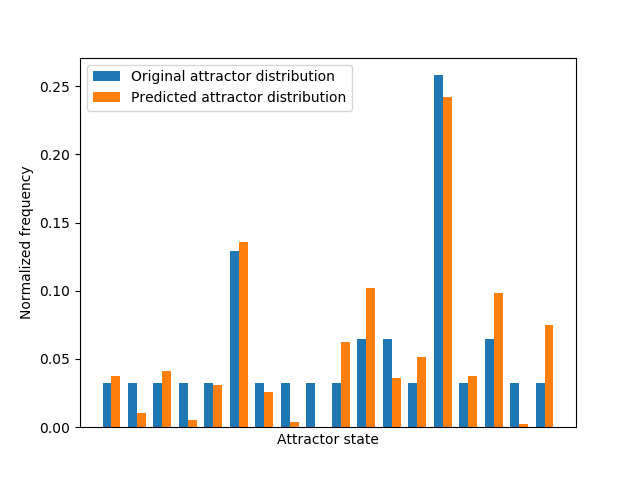
\includegraphics[width=.7\textwidth]{ex9/results.png}
\end{figure}

\question{10}{Considere um modelo de rede Booleana para representar a
saúde de um paciente que descreve o estado de dois genes. Suponha que 
os estados 00 e 10 correspondem respectivamente ao paciente no estado
saudável e doente. Dadas os diagramas abaixo, que representam 
respectivamente a dinâmica dos genes quando o paciente não faz 
tratamento e quando faz, dê a tabela de planejamento para uma janela
de tempo de tamanho 3.}
\begin{center}
\begin{tikzpicture}[node distance=3cm]
  \tikzstyle{state} = [circle, minimum width=20pt, draw, 
  inner sep=0pt, text width=2em, text centered]
    
  % Define nodes
  \node[state] (11) {11};
  \node[state, right of=11] (01) {01};
  \node[state, below of=01] (10) {10};
  \node[state, below of=11] (00) {00};

  \path [->] (11) edge node [above] {$0.5$} (01);
  \path [->] (11) edge node [above left] {$0.5$} (00);
  \path [->] (00) edge [loop below] node [below] {$1.0$} (00);
  \path [->] (01) edge node [left] {$1.0$} (10);
  \path [->] (10) edge [loop below] node [below] {$1.0$} (10);
\end{tikzpicture}
    \hspace{1cm}
\begin{tikzpicture}[node distance=3cm]
  \tikzstyle{state} = [circle, minimum width=20pt, draw, 
  inner sep=0pt, text width=2em, text centered]
    
  % Define nodes
  \node[state] (00) {00};
  \node[state, right of=00] (10) {10};
  \node[state, below of=10] (01) {01};
  \node[state, below of=00] (11) {11};

  \path 
    [->] ([yshift=.1cm]00.east) edge node [above] {$1$} ([yshift=.1cm]10.west)
    [->] ([yshift=-.1cm]10.west) edge node [below] {$0.7$} ([yshift=-.1cm]00.east)
    [->] (11) edge [loop below] node [below] {$1.0$} (00)
    [->] (01) edge node [above] {$0.3$} (11)
    [->] ([xshift=.1cm]10.south) edge node [right] {$0.3$} ([xshift=.1cm]01.north)
    [->] ([xshift=-.1cm]01.north) edge node [left] {$0.7$} ([xshift=-.1cm]10.south);
\end{tikzpicture}
\end{center}

Primeiro, escolhemos o custo dos estados finais do sistema afim de 
encontrar políticas que reduzem este custo.
\begin{center}
\begin{tabular}{c | c }
 $X$ & $C_3(X)$ \\
  \hline
  $00$ & 10 \\
  $01$ & 10000 \\
  $10$ & 10000 \\
  $11$ & 5000 \\
\end{tabular}
\end{center}

Definimos $\mu_i$ como uma variável que indica se houve tratamento no
tempo $i$, e também definimos uma função $J_i$ com os custos parciais 
no tempo $i$.
\begin{align*}
  J_i (X_i, \mu = 1) & = 20 + 10 * i + E [J_{i + 1} (X_{i+1}) | X_i, \mu = 1] \\
  J_i (X_i, \mu = 0) & = 10 + E [J_{i + 1} (X_{i+1}) | X_i, \mu = 0] \\
  J_i (X_i) &= min\{ J_i (X_i, \mu = 0), J_i (X_i, \mu = 1)\}
\end{align*}
Também definimos $J_3 (X) = C_3  (X)$ e $u_i^*(X_i)$ como $1$ se 
$J_i (X_i, \mu = 0) > J_i (X_i, \mu = 1)$ e como $0$ caso contrário. 

Desta maneira, temos que:
\begin{itemize}
  \item{No tempo $i = 2$}
  \begin{align*}
    &J_2 (00, \mu = 0) = 10 + 1.0 * J_3 (00) = 20 \\
    &J_2 (00, \mu = 1) = 40 + 1.0 * J_3 (10) = 10040  \\
    &\text{portanto, } J_2 (00) = 20 \text{ e } \mu_2^* (00) = 0\\
    &\\
    &J_2 (01, \mu = 0) = 10 + 1.0 * J_3 (10) = 10010 \\
    &J_2 (01, \mu = 1) = 40 + 0.7 * J_3 (10) + 0.3 * J_3 (11) = 8540 \\
    &\text{portanto, } J_2 (01) = 8450 \text{ e } \mu_2^* (01) = 1\\
    &\\
    &J_2 (10, \mu = 0) = 10 + 1.0 * J_3 (10) = 10010 \\
    &J_2 (10, \mu = 1) = 40 + 0.7 * J_3 (00) + 0.3 * J_3 (01) = 3047 \\
    &\text{portanto, } J_2 (10) = 3047 \text{ e } \mu_2^* (10) = 1\\
    &\\
    &J_2 (11, \mu = 0) = 10 + 0.5 * J_3 (01) + 0.5 * J_3 (00) =  5015\\
    &J_2 (11, \mu = 1) = 40 + 1 * J_3 (11) = 5040 \\
    &\text{portanto, } J_2 (11) = 5015 \text{ e } \mu_2^* (11) = 0\\
    &\\
  \end{align*}
  
  \item{No tempo $i = 1$}
  \begin{align*}
    &J_1 (00, \mu = 0) = 10 + 1.0 * J_2 (00) = 30 \\
    &J_1 (00, \mu = 1) = 30 + 1.0 * J_2 (10) = 3077 \\
    &\text{portanto, } J_1 (00) = 30 \text{ e } \mu_1^* (00) = 0\\
    &\\
    &J_1 (01, \mu = 0) = 10 + 1.0 * J_2 (10) = 3057 \\
    &J_1 (01, \mu = 1) = 30 + 0.7 * J_2 (10) + 0.3 * J_2 (11) = 3667.4 \\
    &\text{portanto, } J_1 (01) = 3057 \text{ e } \mu_1^* (01) = 0\\
    &\\
    &J_1 (10, \mu = 0) = 10 + 1.0 * J_2 (10) = 3057 \\
    &J_1 (10, \mu = 1) = 30 + 0.7 * J_2 (00) + 0.3 * J_2 (01) = 2579 \\
    &\text{portanto, } J_1 (10) = 2579 \text{ e } \mu_1^* (10) = 1\\
    &\\
    &J_1 (11, \mu = 0) = 10 + 0.5 * J_2 (01) + 0.5 * J_2 (00) = 4245 \\
    &J_1 (11, \mu = 1) = 30 + 1 * J_2 (11) =  5045 \\
    &\text{portanto, } J_1 (11) = 4245 \text{ e } \mu_1^* (11) = 0\\
    &\\
  \end{align*}
  
\item{No tempo $i = 0$}
  \begin{align*}
    &J_0 (00, \mu = 0) = 10 + 1.0 * J_1 (00) = 40 \\
    &J_0 (00, \mu = 1) = 20 + 1.0 * J_1 (10) = 2599 \\
    &\text{portanto, } J_0 (00) = 40 \text{ e } \mu_0^* (00) = 0\\
    &\\
    &J_0 (01, \mu = 0) = 10 + 1.0 * J_1 (10) = 2589 \\
    &J_0 (01, \mu = 1) = 20 + 0.7 * J_1 (10) + 0.3 * J_1 (11) = 3098.8 \\
    &\text{portanto, } J_0 (01) = 2589 \text{ e } \mu_0^* (01) = 0\\
    &\\
    &J_0 (10, \mu = 0) = 10 + 1.0 * J_1 (10) = 2589 \\
    &J_0 (10, \mu = 1) = 20 + 0.7 * J_1 (00) + 0.3 * J_1 (01) = 958.1 \\
    &\text{portanto, } J_0 (10) = 958.1 \text{ e } \mu_0^* (10) = 1\\
    &\\
    &J_0 (11, \mu = 0) = 10 + 0.5 * J_1 (01) + 0.5 * J_1 (00) = 1553.5 \\
    &J_0 (11, \mu = 1) = 20 + 1 * J_1 (11) =  4265 \\
    &\text{portanto, } J_0 (11) = 1553.5 \text{ e } \mu_0^* (11) = 0\\
    &\\
  \end{align*}
\end{itemize}

Portanto, a tabela de planejamento é dada por:
\[
\begin{blockarray}{cccc}
0 & 1 & 2 \\
\begin{block}{(ccc)c}
  0 & 0 & 0 & 00 \\
  0 & 0 & 1 & 01 \\
  1 & 1 & 1 & 10 \\
  0 & 0 & 0 & 11 \\
\end{block}
\end{blockarray}
\]


\end{document}

